\documentclass[../ala_hataile.tex]{subfiles}
\begin{document}

\includepdf[pages=8-9, pagecommand={}]{sisasivut_19062018.pdf}
\twocolumn[\section{Meteorologia}]
\begin{figure*}[!b]
	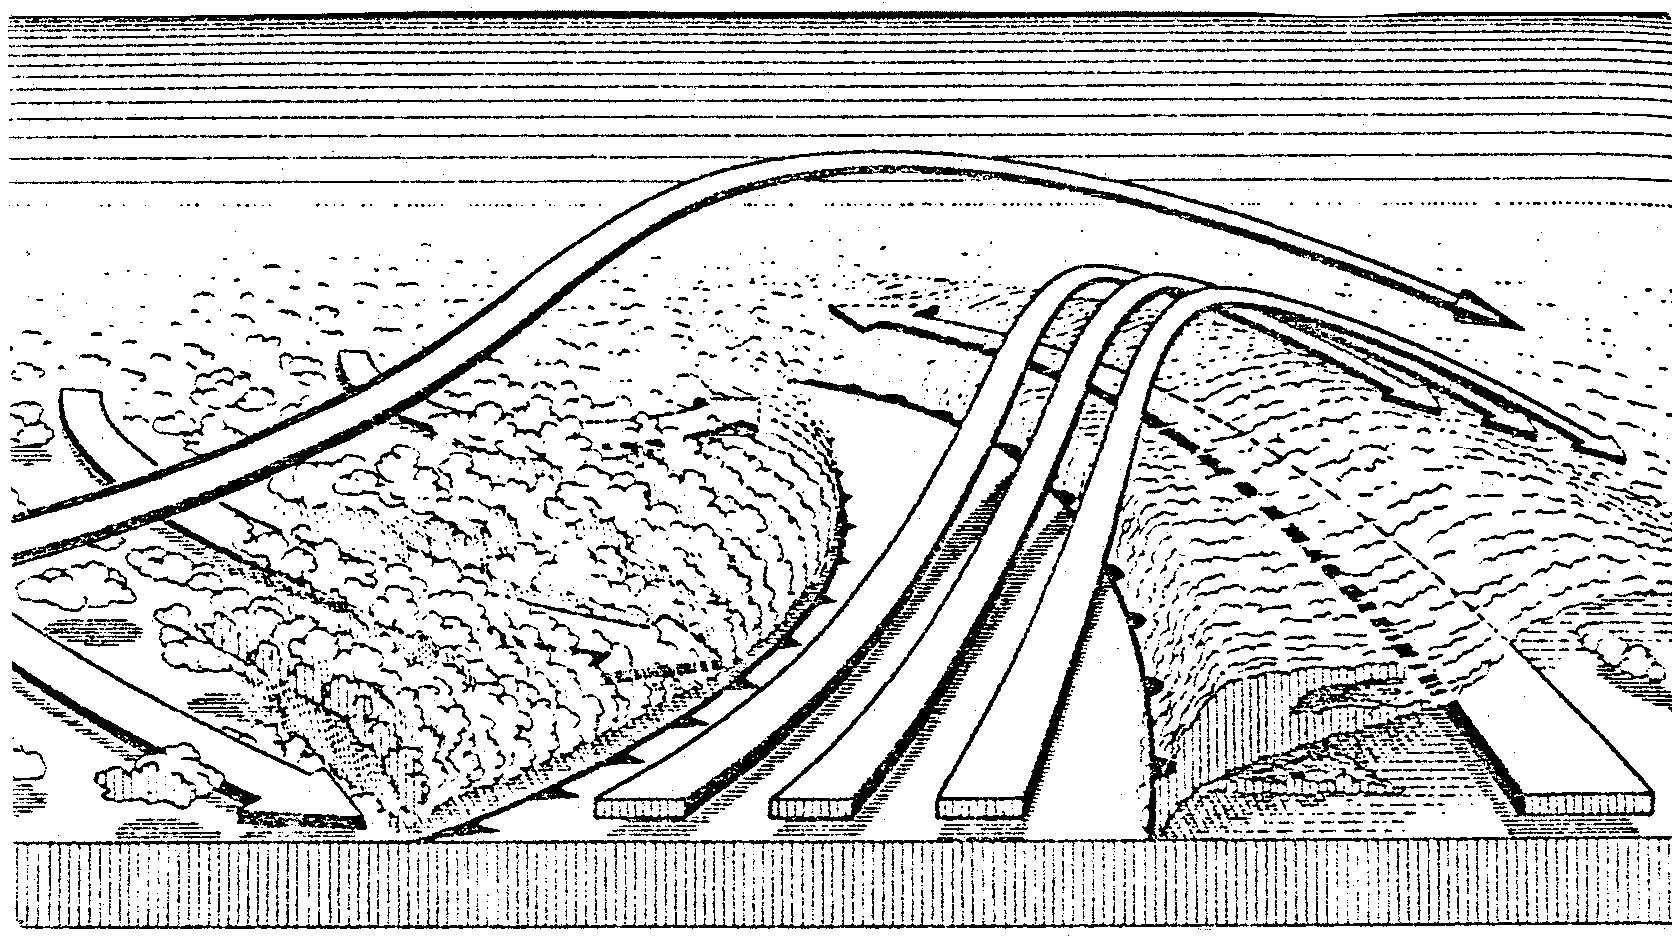
\includegraphics[width=\textwidth]{sykloni.png}
\end{figure*}
Monelle tulee meteorologiasta ensimmäisenä mieleen televisiosta tutut Mette Mannonen ja Pekka Pouta. Todellisuudessa meteorologia on ilmakehän fysiikkaa ja sään ennustus on vain sen tunnetuin sovellus, mutta myös esimerkiksi ilmastonmuutos- ja ilmanlaatukysymysten ratkaisemiseen tarvitaan meteorologeja. Vain hyvin pieni osa valmistuneista meteorologeista valitsee uran television säätiedotteiden parissa. Meteorologiassa tutkitaan ilmakehän ilmiöitä kuten trooppisia hurrikaaneja ja pilvien syntymekanismeja niin havaintojen kuin fysiikan teoriankin avulla. Tietokoneiden käytössä meteorologia on edelläkävijä, ja mm.\,kaaosteoria muotoiltiin paljolti ilmakehää kuvaavia yhtälöitä tarkastelemalla. Nykyaikainen meteorologi onkin laajan tieto- ja taitopohjan omaava tieteen ammattilainen.

Meteorologin tutkintona toimii filosofian maisterin tutkinto. Tutkinnon suorittamisen tavoiteaika on viisi vuotta, ja pääosin valmistuneet ovat suorittaneet opintonsa tässä ajassa. Opinnot koostuvat kahdesta osasta, niin kutsutuista kandi- ja maisterivaiheesta. Kandivaihe tehdään fysikaalisten tieteiden kandiohjelmassa meteorologian opintosuunnalla ja kestää yleensä noin kolme vuotta. Tänä aikana aikana meteorologian opiskelija saa hyvän pohjan fysiikasta ja laajat matemaattiset valmiudet. Kandivaiheen opintoihin kuuluu nykyään myös olennaisena osana datan käsittelyä, ohjelmointia ja tilastollista analyysiä.

Valmistuttuaan luonnon\-tieteiden kandidaatiksi meteorologian opiskelija siirtyy opiskelemaan Ilma\-kehä\-tieteiden maisteri\-ohjelmaan. Maisteri\-ohjelmassa syvennytään ilma\-kehässä tapahtuviin meteorologisiin ilmiöihin yksityis\-kohtaisemmin. Tässä vaiheessa opiskelijat voivat myös painottaa opintojaan eri meteorologian aloihin, kuten suuren mittakaavan dynaamiseen meteorologiaan, sateelliitti\-kauko\-kartoitukseen tai eko\-systeemien ja ilmakehän vuoro\-vaikutusta käsittelevään mikro\-meteorologiaan. Opintojen loppuvaiheessa opiskelija tekee loppu\-työkseen syventävien opintojen tutkielman, joka oikeuttaa filosofian maisterin tutkintoon ja siten meteorologin oppiarvoon.

Suurimmat meteorologien työn\-antajat Suomessa ovat Ilma\-tieteen laitos, Helsingin yliopisto, Vaisala ja Foreca. Näiden lisäksi meteorologeja on työllistyneenä myös tuuli- ja aurinko\-energia-alalla toimivissa konsultti\-yrityksissä ja insinööri\-toimistoissa. Ilmatieteen laitoksella meteorologin on mahdollista työllistyä joko sää\-palvelu\-tuotantoon tai tutkimukseen. Helsingin yliopiston meteorologian tutkintoa arvostetaan myös ulkomailla, joten halutessaan omaa uraansa voi luoda myös muualla maailmassa. Meteorologien työllisyystilanne Suomessa on ollut ja on edelleen hyvä.

Meteorologian opiskelijoiden ainejärjestö on nimeltään Synop~ry. Meitä synoplaisia on vain viitisenkymmentä, mutta olemme sitäkin eloisampi ja aktiivisempi järjestö. Otamme uudet meteorologian opiskelijat lämpimästi mukaan iloiseen joukkoomme!

\vspace{0.5cm}
\noindent\textsc{Sasu Karttunen}
\vspace{1cm}

\subsection*{Meteorologian kursseja}
\subsubsection*{Meteorologian ja säähavainnonteon perusteet (5~op)}
MetPer hyvin perustavanlaatuinen kurssi kaikille
säästä ja sen havainnoinnista kiinnostuneille
fyysikosta filologiin. Kurssilla opitaan
tunnistamaan sääilmiöitä ja käydään
läpi meteorologian peruskäsitteistöä. Osana
suoritusta on myös sääpäiväkirjan teko.
Kurssiin kuuluu myös tutustumiskäyntejä,
muun muassa Ilmatieteen laitokselle. Tällaisesta
yleisön kosiskelusta johtuen kurssi
on yleensä tupaten täynnä.
\subsubsection*{Ilmakehän termodynamiikka (5~op)}
Tällä kurssilla päästään ensimmäistä
kertaa todelliseen ilmakehään kiinni. Viimeistään
tässä vaiheessa kannattaa integrointi
olla hanskassa, muuten kuiva-adiabaattisen
lämpötilavähetteen johtaminen
potentiaalilämpötilan säilymisestä voi tuntua
tuskalliselta. Kurssi on silti mukavaa
ajanvietettä, ja täällä opitaan käyttämään
emagrammia (tästä on oikeasti hyötyä
myöhemmin).
\subsubsection*{Ilmakehän virtausdynamiikan perusteet (10~op)}
Kurssissa on kyse juuri siitä mitä nimi
kertoo. Täällä johdetaan liikeyhtälöt siinä
muodossa, missä meteorologi niitä käyttää
(sori vaan, maapallo nyt sattuu olemaan
pyörivä pallokoordinaatisto). Ison skaalan
dynamiikan lisäksi raapaistaan myös rajakerrosta,
ja selvitetään miksi tähän asti on
aina pitäydytty ``vapaassa ilmakehässä''.
Meteorologin peruskauraa, nämä asiat täytyy
olla hanskassa.

\vspace{0.5cm}\noindent\textsc{Tuomo Lauri}

\subsubsection*{Klimatologian perusteet + Fysikaalinen klimatologia (2+3~op)}
Kurssi johdattaa opiskelijan
klimatologian kiehtovaan maailmaan.
Kurssin alkuosa on
deskriptiivistä eli kuvailevaa
klimatologiaa ja siinä
keskitytään maailman eri ilmasto\-vyöhykkeisiin ja niiden täsmälliseen
luokitteluun. Ja niitä luokkia muuten
on huomattavasti enemmän, kuin mitä lukiomantsan
pohjalta voisi olettaa. Sokerina
pohjalla on myös hauskaa triviaa erilaisista
sääennätyksistä. Matematiikkaa sen paremmin
kuin fysiikkaakaan ei kurssin alkuosalla
juurikaan näy, mutta laskarit pidetään
silti säännöllisesti jok'ikinen viikko.
Kurssin loppuosa keskittyy taas juurikin
siihen fysikaaliseen klimatologiaan ja tutuksi
pitäisivät tulla ainakin erilaiset energian\-siirto\-mekanismit
ja niiden vaikutukset
ilmastoon. Aivan finaalissa päästään raapimaan
myös hieman ilmaston muuttumista
ja siihen vaikuttavia tekijöitä, kuten maan
rataparametrien vaihteluita. Kurssin toinen
osa on kokonaisuudessaan melko työläs ja
ehkä myös hivenen vaikea, mutta toisaalta
kurssipruju on onneksi erinomainen ja
myös luennoitsija on ollut viime vuosina
sieltä paremmasta päästä.

Vaikka kurssi sisältää törkeän määrän
asiaa, kannattaa se kuitenkin suorittaa kunnolla,
sillä palkkioksi saa aimo annoksen
erittäin hyödyllistä ja yleissivistävää tietoa
suuren skaalan ilmastojärjestelmistä. Tämä
on juurikin sitä asiaa, jonka kaikenkarvaiset
sedät, tädit ja papat olettavat juurikin
sinun meteorologian opiskelijana hallitsevan,
sen sään ennustamisen lisäksi tietysti.

\subsubsection*{Kasvihuoneilmiö, ilmastonmuutos ja vaikutukset (5~op)}
Jokamiehen kurssi tarjoaa ajankohtaista
ja mielenkiintoista faktaa kasvihuoneilmiöstä.
Mistä se johtuu, mihin mennään
tulevaisuudessa ja miten tulevaisuutta
ennustetaan. Tällä kurssilla selviää ilman
laajoja esitietoja, joskin yleistietämys meteorologiasta
on hyödyllistä, jos aihealueista
haluaa saada mitään syvällisempää irti.
Kurssista on olemassa erinomainen suomenkielinen
pruju.

\subsection*{Maisteriohjelman maistelukursseja}
\subsubsection*{Boundary Layer Physics I (5~op)}
Boundary Layer Physics~I, eli suomalaisittain Rajakerroksen fysiikka~I, on kurssi jota voi suositella
kyllä kaikille. Dynamiikan kursseilla käsitellään asioita
vapaassa ilmakehässä, jossa ei ole kitkaa
tai muitakaan ikäviä vektorisuureita sotkemassa
tilannetta. Rajakerroksen fysiikka
taas kertoo, mitä tapahtuu vapaan
ilmakehän alapuolella lähellä maanpintaa,
jossa erinäiset turbulenssi-ilmiöt tulevat
häiritsemään kovasti tilannetta. Perinteisesti
rajakerroksen korkeudeksi on määritelty
300~m--3~km, mutta tämä hieman vaihtelee tilanteen
mukaan.

\subsubsection*{Climate change now (2--5~op)}
Climate change now eli suomeksi Ilmastonmuutos nyt on kaikkien alojen opiskelijoille suunnattu kokonaisuus ilmastonmuutoksen perusteista. Kurssin lähestymistapa ilmastonmuutokseen on poikkitieteellinen ja kurssi sopiikin hyvin myös niille, jotka eivät ole fysiikkaa lukiossa lukeneet. Kurssilla hyödynnetään verkkopohjaista oppimisalustaa, joka sisältää mm.\,videoluentoja, "-haastatteluja sekä tehtäviä. Kurssi on mahdollisena suorittaa joko 2 tai 5 opintopisteen laajuisena. 5 opintopisteen suoritukseen vaaditaan oppimispäiväkirjan laatimisen lisäksi kahteen ryhmässä tehtävään projektityöhön osallistumista.

\vspace{0.5cm}
\noindent\textsc{Sasu Karttunen}
\end{document}